\subsection{Auckland}

Al realizar el experimento, se logró llegar al destino en el ttl 22. De estos, 6 no respondieron. Los ttls que Cimbala reconoció como intercontinentales fueron 6, 10, 15, 16, 19, 22.

\begin{figure}[!htbp]
  \centering
    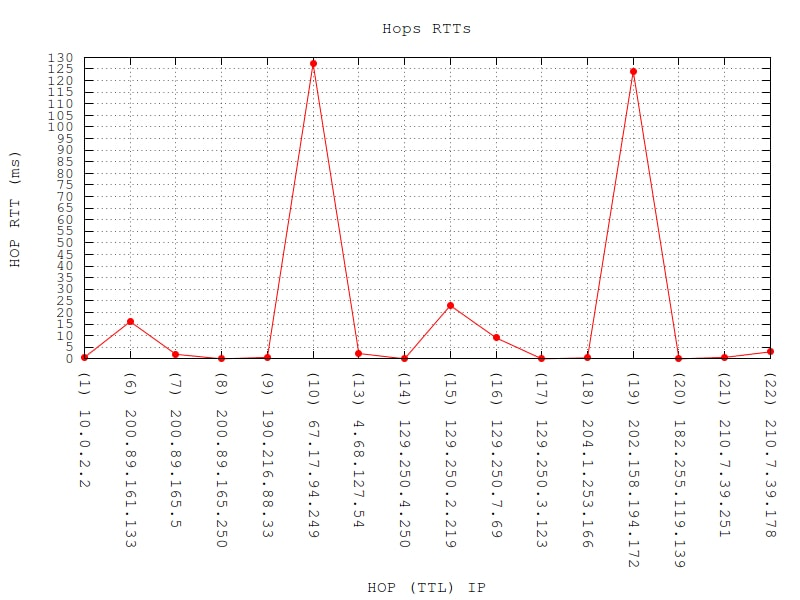
\includegraphics[scale=0.6]{imagenes/auckland-graficos/traceroute-auckland.jpg}
  \caption{auckland- RTT hops}
  \label{fig:7}
\end{figure}

En la figura \ref{fig:7} se puede observar como el ttl 10 y 19 tienen un rtt claramente distinguido del resto.

\begin{figure}[!htbp]
  \centering
    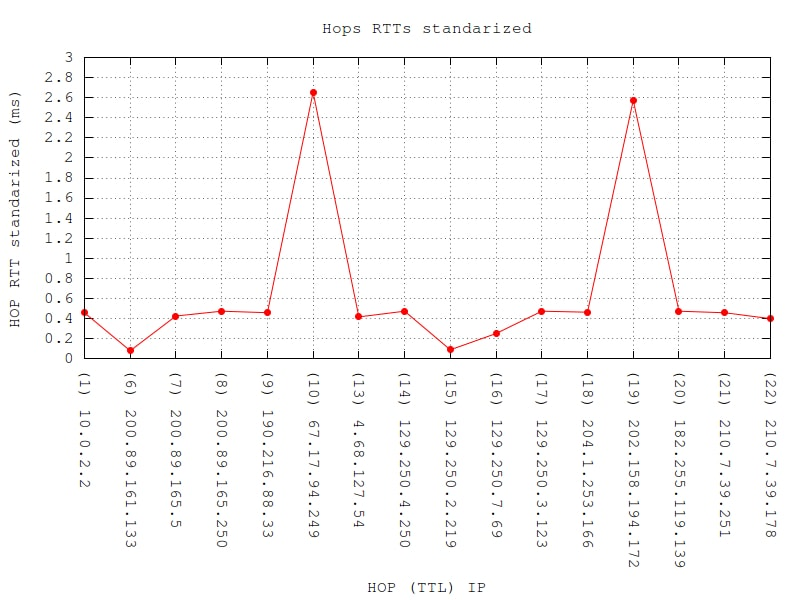
\includegraphics[scale=0.6]{imagenes/auckland-graficos/traceroute-auckland-standarized.jpg}
  \caption{auckland- RTT hops standarized}
  \label{fig:8}
\end{figure}

En la figura \ref{fig:8} se puede observar una situacion similar a la de la figura \ref{fig:7}.


